\title{Nicholas Hunt-Walker Brief Career Biography}
\maketitle

\begin{wrapfigure}{l}{0.225\textwidth}
\vspace{-15pt}
%\begin{center}
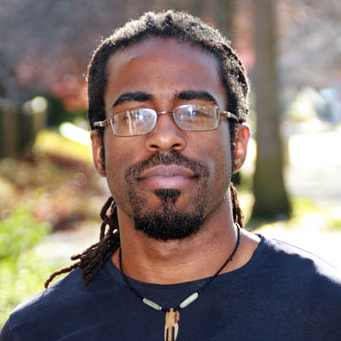
\includegraphics[width=0.2\textwidth]{profile.jpg}
%\end{center}
\vspace{-10pt}
\end{wrapfigure}
\noindent Nicholas discovered his love for physics during his junior and senior years of high school at Elmont Memorial Junior-Senior High School. This continued at the City University of New York (CUNY) at Queensborough Community College when he took his first course in astronomy. This course caused him to change from a major in business administration and transfer to CUNY York College in 2007 to pursue his Bachelor's degree in physics and mathematics. After two and a half years at York, he finished his undergraduate career with the Post-Baccalaureate Program at Columbia University, serving as a researcher in high-energy astrophysics.  In the late summer of 2010 he moved to Seattle, where he began his graduate studies in astronomy at the University of Washington (UW). He has thus far obtained his Masters of Science in astronomy (2012), and is currently in pursuit of his Ph.D.\\

Throughout his journey from Queensborough to UW, Nicholas has been fortunate to have been given many opportunities to learn be a researcher, a presenter, as well as a teacher. In the summer of 2006, his astronomy professor at Queensborough enabled him to perform research looking into solar activity leading up to solar flares, despite not having a major in physics or astronomy. He also tutored for the College Discovery program for a year, assisting students in account, mathematics, and astronomy. While at York College, he was fortunate to take part in a number of research projects in both physics and astronomy. He worked in a lab investigating the properties of water in elastic tissue using Nuclear Magnetic Resonance probes. In the summer 2007 he interned at the Smithsonian Institute's National Air and Space Museum. The summer of 2008 brought him to the American Museum of Natural History as a participant of the National Science Foundation's Research Experiences for Undergraduates (NSF-REU) program. While there, he studied the rate of star formation in distant galaxies. The following summer, he participated in another NSF-REU at the University of Wisconsin, studying exotic X-ray sources in nearby dwarf galaxies. During the year that followed he delved heavily into gamma-ray astronomy on two projects, searching for gamma-ray emission from a distant galaxy with one, and looking for high-energy stellar remnants with another. All the while, he tutored physics, mathematics, and chemistry for freshmen and sophomores at York College. Currently, he is searching for clues to the structure of our own Milky Way galaxy for his Ph.D. thesis, while spending his sixth academic quarter as a teaching assistant for freshmen astronomy classes. 

